%
\documentclass[12pt]{article}

% The usual packages
\usepackage{fullpage}
\usepackage{breakcites}
\usepackage{setspace}
\usepackage{endnotes}
%\usepackage{float} % can't use with floatrow
\usepackage{amsmath}
\usepackage{amsfonts}
\usepackage{amssymb}
\usepackage{rotating}
\usepackage{longtable}
\usepackage{microtype}
\usepackage{graphicx}
\usepackage{hyperref}
%\usepackage[usenames,dvipsnames]{color}
\usepackage{url}
\usepackage{natbib}
\usepackage{framed} 
\usepackage{epigraph}
\usepackage{lipsum}
%\usepackage{dcolumn}
%\restylefloat{table}
\bibpunct{(}{)}{;}{a}{}{,}

% Set paragraph spacing the way I like
\parskip=0pt
\parindent=20pt

%\usepackage{helvet}
\usepackage[labelfont={bf}, margin=0cm, font=small, skip=0pt]{caption}


% Define mathematical results
\newtheorem{lemma}{Lemma}
\newtheorem{proposition}{Proposition}
\newtheorem{theorem}{Theorem}
\newtheorem{claim}{Claim}
\newenvironment{proof}[1][Proof]{\begin{trivlist}
\item[\hskip \labelsep {\bfseries #1}]}{\end{trivlist}}
\newenvironment{definition}[1][Definition]{\begin{trivlist}
\item[\hskip \labelsep {\bfseries #1}]}{\end{trivlist}}
\newenvironment{example}[1][Example]{\begin{trivlist}
\item[\hskip \labelsep {\bfseries #1}]}{\end{trivlist}}
\newenvironment{remark}[1][Remark]{\begin{trivlist}
\item[\hskip \labelsep {\bfseries #1}]}{\end{trivlist}}
\DeclareMathOperator*{\argmin}{arg\,min}
\DeclareMathOperator{\med}{med}
\DeclareMathOperator*{\E}{\text{E}}

%Set up fonts the way I like
\usepackage{tgpagella}
\usepackage[T1]{fontenc}
\usepackage[bitstream-charter]{mathdesign}

%% Baskervald
%\usepackage[lf]{Baskervaldx} % lining figures
%\usepackage[bigdelims,vvarbb]{newtxmath} % math italic letters from Nimbus Roman
%\usepackage[cal=boondoxo]{mathalfa} % mathcal from STIX, unslanted a bit
%\renewcommand*\oldstylenums[1]{\textosf{#1}}

%\usepackage[T1]{fontenc}
%\usepackage{newtxtext,newtxmath}

% A special command to create line break in table cells
\newcommand{\specialcell}[2][c]{%
 \begin{tabular}[#1]{@{}c@{}}#2\end{tabular}}


%% Set up lists the way I like
% Redefine the first level
\renewcommand{\theenumi}{\arabic{enumi}.}
\renewcommand{\labelenumi}{\theenumi}
% Redefine the second level
\renewcommand{\theenumii}{\alph{enumii}.}
\renewcommand{\labelenumii}{\theenumii}
% Redefine the third level
\renewcommand{\theenumiii}{\roman{enumiii}.}
\renewcommand{\labelenumiii}{\theenumiii}
% Redefine the fourth level
\renewcommand{\theenumiv}{\Alph{enumiv}.}
\renewcommand{\labelenumiv}{\theenumiv}
% Eliminate spacing around lists
\usepackage{enumitem}
\setlist{nolistsep}

% Create footnote command so that my name
% has an asterisk rather than a one.
\long\def\symbolfootnote[#1]#2{\begingroup%
\def\thefootnote{\fnsymbol{footnote}}\footnote[#1]{#2}\endgroup}

% Create the colors I want
\usepackage{color}
\definecolor{darkred}{RGB}{100,0,0}

% set up pdf
\hypersetup{
pdftitle={Transformation-Induced Bias}, % title
pdfauthor={Carlisle Rainey}, % author
pdfkeywords={bias} {first difference} {marginal effect} {quantities of interest} {maximum likelihood}
pdfnewwindow=true, % links in new window
colorlinks=true, % false: boxed links; true: colored links
linkcolor=black, % color of internal links
citecolor=black, % color of links to bibliography
filecolor=blue, % color of file links
urlcolor=blue % color of external links
}

% section headers
%\usepackage[scaled]{helvet}
%\renewcommand\familydefault{\sfdefault} 
%\usepackage[T1]{fontenc}
%\usepackage{titlesec}
%\titleformat{\section}
%  {\normalfont\sffamily\Large\bfseries}
%  {\thesection}{1em}{}
%\titleformat{\subsection}
%  {\normalfont\sffamily\large\bfseries}
%  {\thesection}{1em}{}
%  \titleformat{\subsubsection}
%  {\normalfont\sffamily\bfseries}
%  {\thesection}{1em}{}

% enable comments in pdf
\newcommand{\dtk}[1]{\textcolor{blue}{#1}}
\newcommand{\ctk}[1]{\textcolor{red}{#1}}


\begin{document}

\begin{center}
{\LARGE \textbf{Transformation-Induced Bias}}\\\vspace{2mm}
{ \textbf{Unbiased Coefficients Do Not Imply Unbiased Quantities of Interest}}%\symbolfootnote[1]{All computer code necessary for replication is available at \href{https://github.com/carlislerainey/transformation-induced-bais}{github.com/carlislerainey/transformation-induced-bias}.}

\vspace{5mm}

%Carlisle Rainey\symbolfootnote[2]{Carlisle Rainey is Assistant Professor of Political Science, Texas A\&M University, 2010 Allen Building, College Station, TX, 77843 (\href{mailto:crainey@tamu.edu}{crainey@tamu.edu}).}
\end{center}

\vspace{5mm}

% Abstract
{\centerline{\textbf{Abstract}}}
\begin{quote}\noindent
Political scientists commonly focus on quantities of interest computed from model coefficients rather than on the coefficients themselves. 
However, the quantities of interest, such as predicted probabilities, first differences, and marginal effects, do necessarily not inherit the small sample properties of the coefficient estimates. 
Indeed, unbiased coefficients estimates are neither necessary nor sufficient for unbiased estimates of the quantities of interest. 
I characterize this transformation-induced bias, calculate an approximation, illustrate its importance with two simulation studies, and discuss its relevance to methodological research.
 \end{quote}

% Add quote to first page
% \epigraph{}

%\begin{center}
%Manuscript word count: 
%\end{center}

% Remove page number from first page
\thispagestyle{empty}

% Start main text
%\newpage
\doublespace

%\section*{Introduction}

Political scientists use a wide range of statistical models $y_i \sim f(\theta_i)$, where $i \in \{1,..., N\}$ and $f$ represents a probability distribution. 
The parameter $\theta_i$ is connected to a design matrix $X$ of $k$ explanatory variables and a column of ones by a link function $g$, so that $g(\theta_i) = X_i\beta$. 
In the binary logit, for example, $f$ represents the Bernoulli probability mass function and $g$ represents the logit function, so that $y_i \sim \text{Bernoulli}(\pi_i)$ and $\pi_i = \text{logit}^{-1}(X_i\beta)$.

The researcher usually estimates $\beta$ with maximum likelihood (ML), and, depending on the choice of $g$ and $f$, the estimate $\hat{\beta}$ might have desirable small sample properties. 
However, ML does not produce unbiased estimates in general. 
For this reason, methodologists frequently use Monte Carlo simulations to assess the small sample properties of estimators and provide users with rules of thumb about appropriate sample sizes.
For example, the ML estimates of $\beta$ for the binary logit are biased away from zero, leading \citet[p. 54]{Long1997} to suggest that ``it is risky to use ML with samples smaller than 100, while samples larger than 500 seem adequate.''

Although methodologists tend to focus on estimating model coefficients, substantive researchers tend to focus on some other quantity of interest.
A quantity of interest is simply a \textit{transformation} $\tau$ of the model coefficients. 
Examples include marginal effects, first and second differences, predicted probabilities and expected values, and risk ratios \citep{KingTomzWittenberg2000}.

Fortunately, the invariance principle allows the researcher to calculate estimates of the quantities of interest from the coefficient estimates in a principled manner.
The invariance principle states that if $\hat{\beta}$ is the ML estimate of $\beta$, then for any function $\tau$, the ML estimate of $\tau(\beta)$ is $\tau(\hat{\beta})$ (\citealt[pp. 75-76]{King1989}, and \citealt[pp. 320-321]{CasellaBerger2002}).
That is, researchers can simply transform the ML estimates of the model coefficients to obtain an ML estimate of the quantity of interest.
Of course, if $\hat{\beta}$ is a consistent estimator of $\beta$, then $\tau(\hat{\beta})$ must be a consistent estimator of $\tau(\beta)$. 
But the invariance principle raises an important question: Does $\tau(\hat{\beta})$ inherit the small sample properties of $\hat{\beta}$, such as unbiasedness or approximate unbiasedness?
The answer is no; the estimates of the quantities of interest do \underline{not} inherit the small sample properties of the coefficient estimates. 
For example, a sample size of $N = 250$ that produces nearly unbiased coefficient estimates for a probit model can lead to bias in the marginal effect estimates of 25\% or more.

This subtle, yet crucial, point reveals a disconnect between the work done by substantive scholars and that done by methodologists. 
Methodological work tends to focus on obtaining excellent estimates of the model coefficients, while substantive research tends to focus on estimating quantities of interest. 

Much methodological research implicitly suggests that an approximately unbiased coefficient estimate is necessary and/or sufficient for an approximately unbiased estimate of the quantity of interest. 
Classically, \cite{Nagler1994} uses Monte Carlo simulations to assess the small sample properties of the scobit model coefficients, but he focuses on marginal effects and predicted probabilities in his illustrative application. 
Recently, \cite{Nieman2015} uses simulations to assess the small sample properties of the coefficients in his strategic probit with partial observability, but he focuses his illustrative application on the predicted probability of civil war. 
In order to provide more compelling tools for substantive scholars, methodologists must extend their evaluations beyond coefficient estimates to the quantities that substantive researchers typically care about. 

However, the quantities of interest and likely parameter values vary dramatically across substantive applications, making it difficult or impossible for methodologists to formulate general claims about the behavior of the estimators of potential quantities of interest. 
Therefore, substantive researchers must not shy away from studying the behavior of their chosen estimators in particular application, especially given their deep knowledge of the underlying political processes, the appropriate quantities of interest, and the substantive importance of any biases.
Particularly with small sample sizes, large standard errors, and/or highly nonlinear transformations, substantive scholars should consider application-specific simulations to assess the potential for bias.
Closing the gap between methodological and substantive research requires mindful methodological work from both methodologists and substantive scholars.

\subsection*{The Concepts}

As a motivating example, consider the log-linear model 
\begin{equation}
\log (\text{income}_i) = \beta_{cons} + \beta_{edu} \text{education}_i + \epsilon_i \text{,}\nonumber
\end{equation}
where $\epsilon_i \sim N(0, \sigma^2)$, education is measured in years, and income is measured in thousands of dollars. 
Assuming that the researcher uses the correct model, then least squares, which is also the ML estimator, provides the best unbiased estimator of the coefficients $\beta_{cons}$ and $\beta_{edu}$. 
However, the researcher is not likely interested in $\log(\text{income})$, but in income itself. 
In particular, she might want to estimate the median income among those with 20 years of education $\med(\text{income} ~|~ \text{education} = 20) = e^{\beta_{cons} + 20\beta_{edu}}$. 
Because $\med[\log(y)] = \log[\med(y)]$ for a random variable $y$, one might guess that unbiased estimates of $\beta_{cons}$ and $\beta_{edu}$ lead to unbiased estimates of $\med(\text{income} ~|~ \text{education} = 20)$, but that is not the case. 
If we suppose that $N = 10$, $\beta_{cons} = 2.5$, $\beta_{edu} = 0.1$, $\sigma^2 = 1$, and education takes on integers roughly uniformly from 10 to 20, then $\tau(\beta_{cons}, \beta_{edu}) = e^{\beta_{cons} + 20\beta_{edu}} \approx \$90k$. 
A simple Monte Carlo simulation, though, shows that although $\hat{\beta}_{cons}$ and $\hat{\beta}_{edu}$ are unbiased, the estimate of $\med(\text{income} ~|~ \text{education} = 20)$ is strongly biased upward, so that $\E[\tau(\hat{\beta}_{cons}, \hat{\beta}_{edu})] = E(e^{\hat{\beta}_{cons} + 20\hat{\beta}_{edu}}) \approx \$106k$.

A similar, but conceptually distinct issue arrises when researchers want to calculate the \textit{mean} from a log-linear model $\log(y) = X\beta + \epsilon$. 
Many textbooks highlight that $\E[\log(y|X)] \neq \log[\E(y|X)]$, so that $\E(y | X_i) \neq e^{X_i\beta}$ (e.g., \citealt[pp. 212-215]{Wooldridge2013}). 
This inequality follows from a transformation of the random component of the model (i.e., $\epsilon_i$). 
Even if the model coefficients $\beta$ are \textit{known}, then this inequality holds. 
But researchers can easily avoid this issue by using the correct transformation $\E(y | X_i) = e^{X_i\beta + \frac{\sigma^2}{2}}$. However, the bias that interests me flows from a transformation of the \textit{model coefficients}---even if the researcher uses the correct transformation, then $\hat{\tau}$ is biased. 

But how does a simple transformation of unbiased coefficient estimates induce a large bias in the estimate of the quantity of interest?
We usually think about bias as occurring in the model coefficients $\beta$, so that 
\begin{equation}
\text{coefficient bias} = \E(\hat{\beta}) - \beta \text{.}  \nonumber
\end{equation}
But substantive researchers care mostly about bias in the quantities of interest. 
For convenience, I refer to the bias in the quantities of interest as $\tau$-bias, so that
\begin{equation}
\tau\text{-bias} = \E[\tau(\hat{\beta})] - \tau(\beta)\text{.} \nonumber
\end{equation}
$\tau$-bias is more complex and subtle than biases in the coefficients. 
It can be rewritten and decomposed into two components: transformation-induced $\tau$-bias and coefficient-induced $\tau$-bias, so that
\begin{equation}
\text{total } \tau\text{-bias}= \underbrace{ \E[\tau(\hat{\beta})]-  \tau[\E(\hat{\beta})]  }_{\text{transformation-induced}} + \overbrace{  \tau[\E(\hat{\beta})] - \tau(\beta)  }^{\text{coefficient-induced}}\text{.} \nonumber
\end{equation}
Any bias in the coefficients passes through to the quantities of interest in the sense that, if the coefficient estimates are biased, then the transformation of the true coefficient is not equal to the transformation of the average coefficient estimate, so that
\begin{equation}
\text{coefficient-induced } \tau\text{-bias} = \tau[\E(\hat{\beta})] - \tau(\beta) \text{.}\nonumber
\end{equation}
But the transformation \textit{itself} introduces bias as well, so that
\begin{equation}
\text{transformation-induced } \tau\text{-bias} = \E[\tau(\hat{\beta})]-  \tau[\E(\hat{\beta})] \text{.}\nonumber
\end{equation}
Transformation-induced bias occurs because, in general, $h[\E(y)] \neq \E[h(y)]$ for an arbitrary random variable $y$ and function $h$.

Little methodology research explicitly recognizes this transformation-induced $\tau$-bias and less fully appreciates its practical importance. 
Both methodologists and substantive researchers must become more conscientious of transformation-induced $\tau$-bias, which can be much larger than coefficient bias and disappear more slowly as the sample size increases.

\subsection*{A Characterization}

But how can we characterize the direction of this bias? 
For strictly convex and strictly concave transformations, Jensen's inequality enables a straightforward characterization of the direction of the transformation-induced $\tau$-bias. 
This characterization also provides the key intuition for more complicated transformations.
\begin{theorem}\label{thm:direction}
Suppose a non-degenerate estimator $\hat{\beta}$. Then any strictly convex (concave) $\tau$ creates upward (downward) transformation-induced $\tau$-bias.
\end{theorem} 
\begin{proof}
The proof follows directly from Jensen's inequality. 
Suppose that the non-degenerate sampling distribution of $\hat{\beta}$ is given by $S_\beta(b)$ so that $\hat{\beta} \sim S_\beta(b)$. 
Then $\E(\hat{\beta}) = \int_{B}bS_\beta(b)db$ and $\E[\tau(\hat{\beta})]  = \int_{B}\tau(b)S_\beta(b)db$. 
Suppose first that $\tau$ is convex. 
By Jensen's inequality, $\int_{B}\tau(b)S_\beta(b)db > \tau \left[ \int_{B}bS_\beta(b)db \right]$, which implies that $\E[\tau(\hat{\beta})] > \tau[\E(\hat{\beta})]$. 
Because $\E[\tau(\hat{\beta})] - \tau[\E(\hat{\beta})] > 0$, the transformation-induced $\tau$-bias is upward. 
By similar argument, one can show that for any strictly \textit{concave} $\tau$, $\E[\tau(\hat{\beta})] - \tau[\E(\hat{\beta})] > 0$ and that the transformation-induced $\tau$-bias is downward. $\blacksquare$
\end{proof}

In general, researchers do not restrict themselves to a strictly convex or strictly concave $\tau$.  
This situation is much more difficult to characterize generally because $\tau(b)$ might contain a mixture of convex and concave regions. 
For example, typical transformations of logistic regression coefficients, such as predicted probabilities, first and second differences, marginal effects, and risk ratios, all have both convex regions and concave regions.
Making matters even more difficult, at any particular point $b$, the multivariate function $\tau$ might be convex in one direction and concave in another. 
In general, though, the direction of the bias depends on the \textit{location} of the sampling distribution. 
But the intuition from Theorem \ref{thm:direction} is clear.
If most of the sampling distribution is located in a mostly concave region, then the bias will be downward. 
If most of the sampling distribution is located in a mostly convex region, then the bias will be upward.\footnote{One might wonder about the relevance of these ideas to Bayesian analyses. 
Indeed, the researcher can usually use MCMC to sample directly from posterior of the model coefficients and, by simple extension, sample the quantity of interest from the posterior distribution. 
But if the researcher uses the posterior mode as the point estimate, then the identical logic applies. 
For an alternative point estimate (e.g., posterior mean), the invariance principle no longer holds, so the argument breaks down (i.e., the point estimate of $\tau(\beta)$ is not longer $\tau(\hat{\beta})$. 
However, regardless of the point estimate the researcher uses, a Bayesian approach does not guarantee an unbiased quantity of interest.}

\subsection*{An Approximation}

While the intuition developed by Theorem \ref{thm:direction} helps us understand the \textit{direction} of the bias, how can we assess the \textit{magnitude} of the transformation-induced $\tau$-bias? 
To approximate the magnitude, I use a a second-order Taylor expansion. 
First, notice that $\E[\tau(\hat{\beta})] = \E[\tau(\E[\hat{\beta}] + (\hat{\beta} - \E[\hat{\beta}]))]$. 
Now approximate the term inside the right-hand expectation with a second order Taylor expansion, so that 
\small
\begin{equation}
E[\tau(\hat{\beta})] \approx \E \bigg[ \tau[\E(\hat{\beta})] + \displaystyle \sum_{r = 1}^{k+1} \dfrac{\partial \tau[\E(\hat{\beta})]}{\partial \beta_r}[\hat{\beta}_r - \E(\hat{\beta}_r)] +  \dfrac{1}{2} \displaystyle \sum_{r = 1}^{k+1} \sum_{s = 1}^{k+1} \overbrace{\dfrac{\partial^2 \tau[\E(\hat{\beta})]}{\partial \beta_r \beta_s}}^{\text{Hessian} = H_{rs}}\overbrace{[\hat{\beta}_r - \E(\hat{\beta}_r)][\hat{\beta}_s - \E(\hat{\beta}_s)]}^{\text{Cov}(\hat{\beta}_r, \hat{\beta}_s) = \Sigma_{rs}}  \bigg]\nonumber
%\E[\tau(\hat{\beta})] & \approx \E[\tau(\beta)]  + \dfrac{1}{2} \displaystyle \sum_{r = 1}^{k+1} \sum_{s = 1}^{k+1} H_{rs} \Sigma_{rs}\text{,} \no number
\end{equation}
\normalsize
Taking the expectation of the right-hand side eliminates the middle term and allows expressing the final term as a function of the variance of the sampling distribution, so that 
\begin{equation}
\E [\tau(\hat{\beta})] \approx  \tau[\E(\hat{\beta})]  + \dfrac{1}{2} \displaystyle \sum_{r = 1}^{k+1} \sum_{s = 1}^{k+1} H_{rs} \Sigma_{rs}\text{,} \nonumber
\end{equation}
where $H$ represents the Hessian matrix of second derivatives of $\tau$ at the point $\E(\hat{\beta})$ and, conveniently, $\Sigma$ represents the covariance matrix of the sampling distribution. 
Rearranging gives an approximation to the magnitude of the transformation-induced $\tau$-bias, so that 
\begin{equation}\label{eqn:bias}
\text{transformation-induced } \tau\text{-bias} = \E[\tau(\hat{\beta})] - \tau[\E(\hat{\beta})]  \approx \dfrac{1}{2} \displaystyle \sum_{r = 1}^{k+1} \sum_{s = 1}^{k+1} H_{rs} \Sigma_{rs}\text{.} \nonumber
\end{equation}
If $H$ is constant then the approximation is exact. 
If $\hat{\beta}$ is unbiased, then $\tau[\E(\hat{\beta})]$ can be replaced with $\tau(\beta)$, so that Equation \ref{eqn:bias} represents both transformation-induced and the total $\tau$-bias.

Equation \ref{eqn:bias} does not depend on a strictly convex or concave transformation. 
As long as $\tau$ is not highly non-linear (e.g., $\left|\frac{\partial^3 \tau}{\partial \beta_r \partial \beta_s \partial \beta_t}\right| \approx 0$), then Equation \ref{eqn:bias} provides a reasonable estimate of the direction and magnitude of the bias.

Equation \ref{eqn:bias} quantifies two intuitions. 
First, the amount of bias depends on the standard error or sample size. 
As the sample size grows large, $\Sigma_{rs}$ shrinks to zero, which drives the bias to zero as well. 
This matches the previous observation that $\tau(\hat{\beta})$ is a consistent estimator of $\tau(\beta)$. 
Secondly, the amount of bias depends on the curvature in $\tau$. 
If $\tau$ is nearly linear so that $H \approx 0$, then the transformation introduces minimal bias. 
On the other hand, more curvature, so that $H >> 0$, leads to a large bias. 

\subsection*{Two Monte Carlo Simulations}

But does this bias matter in practice? The following two Monte Carlo studies illustrate the importance of accounting for transformation-induced bias when evaluating estimators. 
Approximately unbiased coefficients are not enough---one must assess the bias in the quantities of interest as well. 

\subsubsection*{A Hypothetical Model}

Many substantive researchers realize that logistic regression estimates are biased away from zero in small samples and use ``rules of thumb'' to judge whether asymptotic properties, such as asymptotic unbiasedness, approximately apply to a finite sample.
When non-events outnumber events, one such rule of thumb requires ten events per explanatory variable \citep{Peduzzietal1996}.
I show that this rule works quite well choosing a sample size that yields approximately unbiased coefficients, but severely underestimates the sample size needed for approximately unbiased estimates of the marginal effects.

For simplicity, I focus on the model $\Pr (y) = \text{logit}^{-1}(\beta_{cons} + \beta_1x_1 + \beta_2x_2 + \beta_3x_3 + \beta_4x_4 + \beta_5x_5 + \beta_6x_6)$, where $y$ indicates whether or not each observation experiences an event and the $x_j$ represent fixed explanatory variables that I create by simulating from independent, standard normal distributions. 
For this simulation, I set $\beta_{cons} = -1$ and $\beta_j =  0.15$ for $j \in \{1, ..., 6\}$. 
I assume that ``approximately unbiased'' means a bias of less than three percent, where
\begin{equation}\label{eqn:percent-bias}
\text{percent bias} = 100 \times \frac{E[\tau(\hat{\beta})] - \tau(\beta)}{\tau(\beta)}\text{.}
\end{equation}
I vary number of observations $N$ from 100 to 3,000, and, for each sample size, I simulate 100,000 data sets, use each data set to estimate the coefficients, and use the estimated coefficients to calculate the marginal effects.
I use these 100,000 estimates to calculate the percent bias given by Equation \ref{eqn:percent-bias}.

Figure \ref{fig:bias-coef} shows the bias in the coefficients as the sample size increases. The left panel shows the bias in $\hat{\beta}_{cons}$ and the right panel shows the bias in $\hat{\beta}_1$. 
For $N = 100$, $\hat{\beta}_{cons}$ and $\hat{\beta}_1$ are biased away from zero by about ten percent. 
However, this bias drops to about three percent for $N = 250$ and nearly disappears for $N = 3,000$. 
The rule of thumb works well; the bias is negligible for about $N = 219$.

\begin{figure}[h!]
\begin{center}
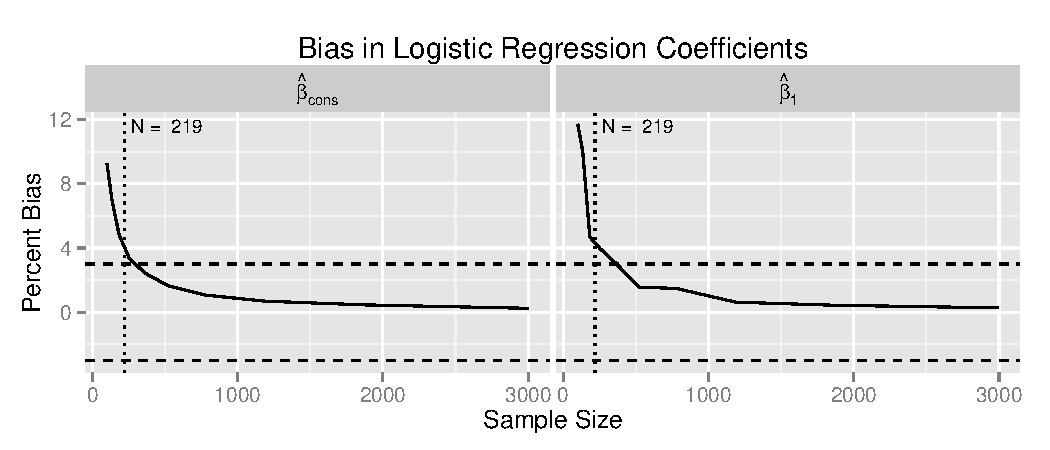
\includegraphics[scale = 0.7]{figs/bias-coef.pdf}
\caption{This figure shows the percent bias for the intercept and coefficient for $x_1$. 
The rule of thumb requiring ten events per explanatory variable suggests a minimum sample size of about 219. 
For samples larger than about 250, the bias falls below three percent and it nearly disappears as the sample size approach 3,000.}\label{fig:bias-coef}
\end{center}
\end{figure}

Figure \ref{fig:bias-me} shows the bias in the estimates of the marginal effects as the sample size increases. 
The left panel shows the total bias, the middle panel shows the coefficient-induced bias, and the right panel shows the transformation-induced bias.
Since the marginal effect of $x_1$ varies with $x_1$ itself, I plot the estimates for a range of values of $x_1$. 

Two features stand out. 
First, small sample bias is much larger for the marginal effects than for the coefficients. 
For $N = 100$, the estimate of the marginal effect is biased by about -75\% for $x_1 = -3$, -50\% for $x_1 = -2$, and -25\% for $x_1 = -1$. 
Second, the small sample bias in the estimates of the marginal effects descends to zero more slowly than the coefficient estimates.
While the coefficient estimates are approximately unbiased for about $N = 250$, the estimates of the marginal effects retain substantial bias. 
Indeed, the bias in the estimates of the marginal effects drops below the 3\% threshold at about $N = 3,000$---more than ten times the rule of thumb that works well for the coefficients. 

\begin{figure}[h!]
\begin{center}
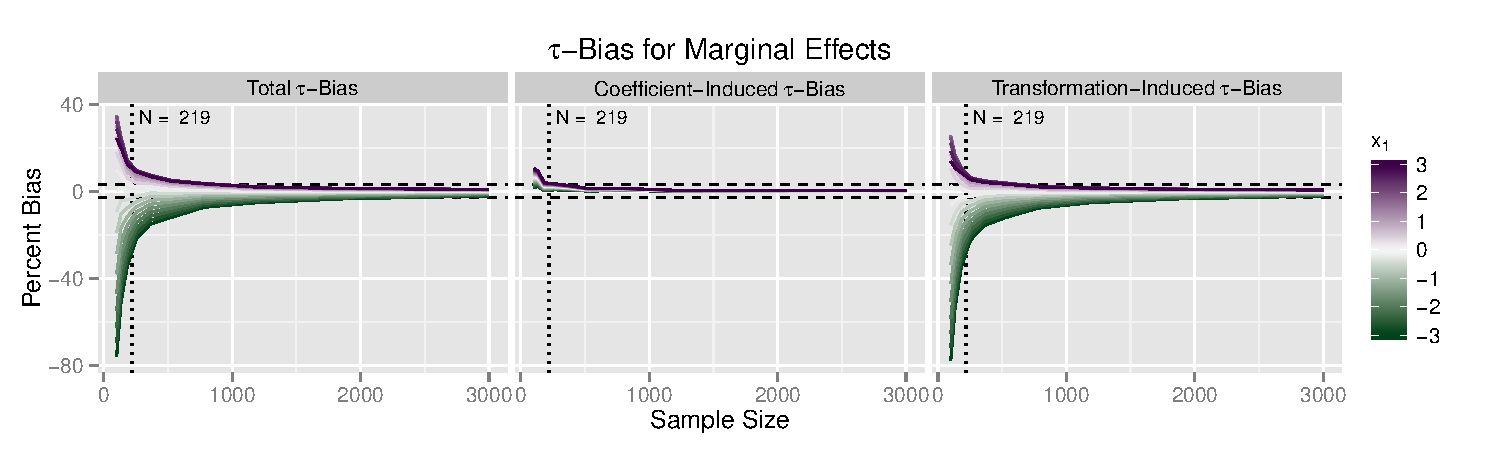
\includegraphics[width = \textwidth]{figs/bias-me.pdf}
\caption{This figure shows the total, coefficient-induced, and transformation-induced $\tau$-bias for the marginal effects. The rule of thumb requiring ten events per explanatory variable suggests a minimum sample size of about 219. However, the bias falls well outside the three percent threshold for this suggested sample size. The estimates fall within the three percent threshold only for sample sizes nearing 3,000---more than ten times the rule of thumb that works well for the coefficients. Also notice that while the coefficient-induced bias receives the most attention from methodologists, the transformation-induced bias is \textit{much} larger.}\label{fig:bias-me}
\end{center}
\end{figure}

\subsubsection*{An Actual Model}

To further highlight the practical implications of transformation-induced $\tau$-bias, I use the explanatory variables and coefficients reported for Model 1 in Table 2 of \citet[p. 286]{Lacina2006} to conduct a second simulation. 
Lacina uses a normal-linear regression model with a log-transformed outcome variable to assess several hypotheses about the causes of the number of battle deaths in civil conflicts.
Using her reported coefficients as the true model parameters and her explanatory variables the predictors (105 complete observations; 9 explanatory variables), I repeatedly (1) simulate a new outcome variable, (2) re-estimate the regression model, and (3) calculate the quantities of interest.
For each set of estimates $\hat{\beta}$ and $\hat{\sigma}^2$, I calculate two quantities of interest:
\begin{enumerate}
\item The expected number of battle deaths $E(\text{deaths}_i~|~X_i) = e^{X_i\hat{\beta} + \frac{\hat{\sigma}}{2}}$ for each observed case $X_i$.
\item The first difference (i.e., the change in the expected number of battle deaths) $\Delta(\text{deaths}_i~|~X^{D}_i,~ X^{\sim D}_i)  = E(\text{deaths}_i~|~X^{D}_i) - E(\text{deaths}_i~|~X^{\sim D}_i) =  e^{X_i^{D}\hat{\beta} + \frac{\hat{\sigma}}{2}} - e^{X_i^{\sim D}\hat{\beta} + \frac{\hat{\sigma}}{2}}$ if each observed case $X_i$ were changed from a non-democracy $X^{\sim D}_i$ to a democracy $X^{D}_i$.
\end{enumerate}
Because the estimates of $\beta$ and $\sigma^2$ are unbiased, there is no coefficient-induced $\tau$-bias. 
Indeed, the least squares estimate of $\beta$ is the best unbiased estimator under the assumed normal-linear model. 
However, this ideal small-sample property does not apply to the quantities of interest.
Figure \ref{fig:lacina} summarizes these simulations and demonstrates that transformation-induced $\tau$-bias can create considerable bias in the quantities of interest even when coefficient estimates have optimal properties.

The left panel of Figure \ref{fig:lacina} shows the true value and percent bias for the expected number of battle deaths $E(\text{deaths}) = e^{X\hat{\beta} + \frac{\hat{\sigma}^2}{2}}$. 
Because the estimates $\hat{\beta}$ and $\hat{\sigma}^2$ are unbiased, there is no coefficient-induced $\tau$-bias in the expected value.
However, there is a substantial upward bias in the expected value due to transformation-induced $\tau$-bias.
The upward bias in the expected value ranges from 4\% (307 deaths) to 37\% (51,120 deaths).
The average upward bias is 10\%---these are not trivial biases.

The right panel of Figure \ref{fig:lacina} shows that these upward biases do not cancel for the first difference. 
Indeed, transformation-induced $\tau$-bias leads to an overly optimistic estimate of the effect of democracy. 
Lacina correctly notes that ``democracy is associated with fewer battle deaths'' (p. 287), but transformation-induced $\tau$-bias might lead researchers to over-estimate this pacifying effect by up to 10\% (and about 35\% in one extreme case) and 6\% on average.

\begin{figure}[h!]
\begin{center}
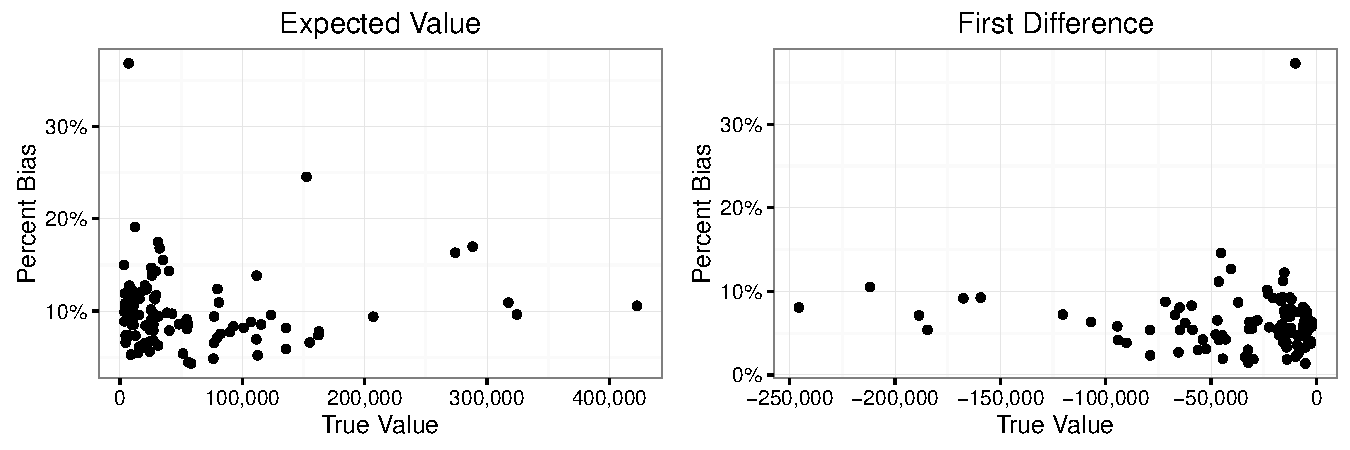
\includegraphics[scale = .7]{figs/lacina.pdf}
\caption{This figure shows the transformation-induced $\tau$-bias for two quantities of interest. Each point represents a single observation from Lacina's (\citeyear{Lacina2006}) data set. For each observation, I calculate the transformation-induced $\tau$-bias in the expected value---the expected number of battle deaths---and in the first difference---the change in the expected number of deaths if each case was changed from a non-democracy to a democracy.}\label{fig:lacina}
\end{center}
\end{figure}

\subsection*{The Implications}

Quantities of interest do not inherit the small sample properties of the coefficient estimates. 
This fact has important implications for how we evaluate the small sample properties of estimators. 

First, $\tau$-bias has important implications for the sample sizes that methodologists recommend to substantive researchers. 
Methodologists usually parameterize models so that the coefficients lie in an unbounded space. 
This allows the coefficient estimates to rapidly approach their asymptotic distribution, which ensures the estimates have acceptable small sample properties. 
Substantive researchers, though, usually transform these coefficient estimates into a quantity of interest, which, because it often lies in a bounded space, might approach its asymptotic distribution more slowly. 
As a result, substantive researchers might need much larger sample sizes than methodologists usually recommend. 
Methodologists must remain conscientious of the quantities of interest to substantive researchers and assess the performance of their estimators in terms of these quantities.
Unfortunately, it remains impossible or difficult to assess the bias in general or for a wide range of sample sizes, quantities of interest, or parameter values.

But substantive researchers must also remain aware of the potential to introduce bias into estimates by transforming coefficient estimates. 
Fortunately, substantive researchers can use Monte Carlo simulations to quickly assess the potential for bias in a specific substantive context in which researchers know the sample size, quantity of interest, and likely parameter values. 

Secondly, $\tau$-bias has important implications for the bias-variance tradeoff in choosing an estimator. 
Methodologists usually recognize a tradeoff between bias and variance in estimating parameters. 
Actions intended to remove bias might increase variance and vice versa.
However, the approximation to the transformation-induced $\tau$-bias given in Equation \ref{eqn:bias} points out an important result. 
Greater variance in the coefficient estimates might lead to increased bias in the quantities of interest. 
This implies that if an estimator is essentially unbiased, then greater efficiency translates to reduced bias in the quantities of interest. 
Similarly, small reductions in bias at the expense of a large increase in variance might lead to greater bias in the quantities of interest. 
For example, refinements of the usual logit model intended to \textit{reduce} bias in the coefficients, such as heteroskedastic probit or scobit, might actually \textit{increase} bias in the quantities of interest. 
Methodologists must be aware of this tradeoff when recommending more complex estimators to substantive researchers and comparing alternative estimators.

Methodologists cannot ignore transformation-induced bias. Substantive researchers must not assume that sample size recommendations remain valid for any quantity of interest. Nearly unbiased estimates of coefficients are not enough. We must remain thoughtful about our quantities of interest and calibrate our tools for these quantities.



\singlespace 
%\newpage
\small
\bibliographystyle{apsr_fs}
\bibliography{/Users/carlislerainey/Dropbox/papers/bibliography/bibliography.bib}

\end{document}


















